\documentclass[a4paper]{report}
\usepackage{tikz}
\usepackage[margin=2.5cm]{geometry}
\usepackage{hyperref}
\usepackage{graphicx}
\graphicspath{{figures/}{anotherFigureDirectory/}}
\graphicspath{ {./images/} }
\usepackage{listings}
\usepackage{wrapfig}
\usepackage{color}
\definecolor{bluekeywords}{rgb}{0.13,0.13,1}
\definecolor{greencomments}{rgb}{0,0.5,0}
\definecolor{turqusnumbers}{rgb}{0.17,0.57,0.69}
\definecolor{redstrings}{rgb}{0.5,0,0}
\definecolor{gray}{rgb}{0.13,0.13,0.13}
\lstdefinelanguage{FSharp}
                {morekeywords={let, new, match, with, rec, open, module,
                namespace, type, of, member, and, for, in, do, begin, end, fun,
                function, try, mutable, if, then, else},
                keywordstyle=\color{bluekeywords},
                sensitive=false,
                numbers=left,  % where to put the line-numbers;(none, left, right)
                numberstyle=\tiny\color{gray},
                morecomment=[l][\color{greencomments}]{///},
                morecomment=[l][\color{greencomments}]{//},
                morecomment=[s][\color{greencomments}]{{(*}{*)}},
                morestring=[b]",
                showstringspaces=false,
                stringstyle=\color{redstrings}
                }

\title{PoP - Ugeopgave 7}
\author{Christoffer, Inge og Pernille}
\date{\today}

\begin{document}
\maketitle
\tikzstyle{block} = [rectangle, draw, fill=blue!20, text centered,
    rounded corners, minimum height=2.5em]
\tikzstyle{cloud} = [rectangle, draw, fill=white, text centered,
    rounded corners, minimum height = 2em]
\tikzstyle{line} = [draw, -latex]

\section*{Preface}
As a part of the Programming and Problem Solving course, we,
three Computer Science students at Copenhagen University, build the game Awari.

\section*{Awari}
Awari is an ancient two player game that resembles the beloved Kalaha. The main
objective of Awari is to capture the most beans. The game consists of a board
with 6 pits and one home pit for each player. Each of the 6 x 2 pits consists of
3 beans. The players must in turn take the amount of beans from a pit on his or
her side of the board and distribute them in the following pits. The game
continues until one of the two players has no beans left, and the winner is the
player who captured the most beans in his or her homepit.

\section*{Problem description}
We have implemented the Awari using the functional programming language F\#. We
were given two functions as a start, a turn and a play function, and a signiture
file with type indication for several minor functions. To be able to play the
game we have created functions to print the board, to distribute the beans, to
check for game over etc. All the functions will be elaborated in this rapport.

\begin{figure}
\centering
\begin{tikzpicture} [node distance = 1.5 cm, auto]
		\node [cloud] (start) {The board is printed};
        \node [cloud, below of=start] (choise) {A player chooses a pit};
        \node [cloud, below of=choise] (distribute) {Beans are distributed};
        \node [cloud, below of=distribute] (eval) {The result is evaluated};
		\node [cloud, right of=eval, node distance = 4.5 cm]
            (newp) {The other players turn};
        \node [cloud, left of=eval, node distance = 4 cm]
            (end) {The game is over};
        % Arrows
        \path [line] (start) -- (choise);
        \path [line] (choise) -- (distribute);
        \path [line] (distribute) -- (eval);
        \path [line] (eval) -- (newp);
        \path [line] (newp) |- (start);
        \path [line] (eval) -- (end);

\end{tikzpicture}
\caption{Flow of Awari}
\label{fig:gameflow}
\end{figure}

\section*{Problem analysis and design}
\subsection*{Game board and flow}
We designed our programme starting by focusing on the game board. The board is
the center of the game and thus the main part of our functions takes the board 
as input and returns a new board or evaluates the pits at the board. Figure 1 
illustrates the simple flow of the game. The board with the correct number of beans in each of the pit is the starting point. In the real physical game, you start by setting op the game board to play by putting beans in the pits. The virtual conterpart is printing the board. Here after, the players starts playing beginnig by Player1 picks a pit. As we see from Figure
\ref{fig:gameflow}) the player returns to the printed board after every turn. Based on this, we started by creating our board. It consists of an int array with 14 
integers whereas two are home pits and six pits for each player. As an array 
is mutable we preferred this type to lists. 

\subsection*{Design and user interface}
The design of the game board was important to us. We wanted the gui design to be nice and simple and intuitive to the player. Therefore we started by focusing on the 
\texttt{printBoard} function. 

\begin{wrapfigure}{r}{0.75\textwidth}
\centering
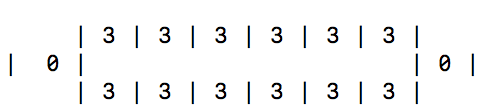
\includegraphics[width=0.60\textwidth]{board1}
\caption{Board of Awari}
\end{wrapfigure}
It prints the array formed as a game board. This makes it clear to the player that it is a game board an not just an array of integers. All the pits are clearly divided and the home pits are situated at each end of the board. We thought that the screen got cluttered with the compiling code and all the printed boards. Therefore we added the \texttt{System.Console.Clear} function to make the terminal look more as a game screen.
\newline
\begin{wrapfigure}{l}{0.75\textwidth}
\centering
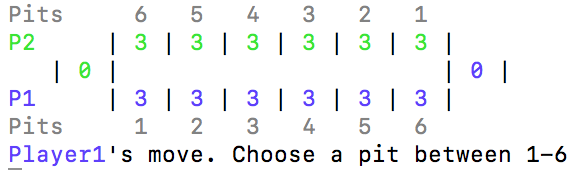
\includegraphics{boardcolor}
\caption{Board of Awari with colour}
\end{wrapfigure}
 
We still suspected that the players could be confused about which pits and 
which side of the board game belonged to who. Therefore we added colours to the
pits and the players: Player 1 is blue and has the blue pits. Player 2 is green
 and has the green pits. In addition, we added the numbers of the pits so to 
not to get confused of which pit is which and in which direction the game is played.

\subsection*{The Players}
The game is played by two players. We have created a type player consisting of a player1 and player2. It is important to distinguish between the two as they have each their home pit and each their side of the board, meaning that they have a specific index as their pits. Player1 has index 0-5 and has homepit in index 6. Player2 has index 7-12 and home pit in index 13. To solve this issue, we made a function \texttt{isHome} that was able to recognize which home pit belonged to each of the players. 

We also needed to know the player's choice of pit from which he or she wanted to take beans. We decided that it should be possible for each player to enter a number on the keyboard between 1-6 and then the game had to convert it to the correct index number, instead of just letting the player know which index numbers belong to him or her. We created the function \texttt{getMove} to sove this problem. It matches the player and the input from a pressed keyboard and returns an index.

\subsection*{Playing the game}

Another function we focused on was the \texttt{distribute} 
function as it distributes the beans taken from a pit and placed in the following. Thereby it updates the board and secure the flow in the game.
\begin{wrapfigure}{l}{0.9\textwidth}
\centering
\begin{tikzpicture} [node distance = 1.5 cm, auto]
		\node [cloud] (start) {3-3};
        \node [cloud, below of=start] (choise) {3+1};
        \node [cloud, below of=choise] (distribute) {2+1};
        \node [cloud, below of=distribute] (eval) {0+1};
		\node [cloud, right of=eval, node distance = 4 cm]
            (newp) {if Home, try again};
        \node [cloud, left of=eval, node distance = 4 cm]
            (end) {If empty, check opposite};
        % Arrows
        \path [line] (start) -- (choise);
        \path [line] (choise) -- (distribute);
        \path [line] (distribute) -- (eval);
        \path [line] (eval) -- (newp);
        \path [line] (eval) -- (end);

\end{tikzpicture}
\caption{Example of the distribute function}
\end{wrapfigure}
\\\\
\\\\
\\\\
\\\\
\\\\
\\\\
\\\\
\\\\
\\\\
Figure 4 illustrates an example of the distribute function, where it takes the 3 beans from the chosen pit and places them in the following. It is a bit more complex than this which is elaborated int the section about functions. 

\section*{Program description}
\subsection*{Types}
From the assignment we've been given som essential types, which were needed to set some game-specified types used in nearly every single game function.

\subsubsection*{board}
The type \texttt{board} takes the fsharp-type \textsl{int array} and is used to create the board of the game representing 12 general pits and 2 home pits, i.e. at set of 6 generals and 1 home per. player.

\subsubsection*{player}
The type \texttt{player} is simply created to make it possible for a function to take the type as an argument. The type has two possible versions \textsl{Player1} or \textsl{Player2}.
\subsection*{Globals}
For showing the colours of players and their pits at the printed game board, we have defined \texttt{player1Color} and \texttt{player2Color}. We use \texttt{pitNumberColor} as the colour of the pits numbers, and \texttt{gameOverColor} is used when the game terminates it write Game Over.
\\\\
We have also defined beginner board, \texttt{board}, with the type array.

\subsection*{isGameOver}
{\it This function is used by \texttt{turn} and \texttt{play}.}
\lstinputlisting[language=FSharp, firstline=143, lastline=147]{AwariLib.fs}
The function takes a board as input and returns a boolean. It returns true if either side of the board has no beans. It is called by \texttt{turn} to check whether the game is over, if it returns True, the whole game terminates.

\subsection*{isHome} 
{\it This function is used by \texttt{turn}.}
\lstinputlisting[language=FSharp, firstline=160, lastline=164]{AwariLib.fs}
The function checks whether a given pit is the home pit for one of the players. It is a boolean type and returns true if it is so.
It is called by \texttt{turn} to a given board, the finalPitsPlayer and the finalPit. If it does not return true in this context, \texttt{turn} returns a new board and the game continues. Else, it calls \texttt{repeat} again with the same player.

\subsection*{getMove} 
{\it This function gets a player's next move.}
\lstinputlisting[language=FSharp, firstline=176, lastline=195]{AwariLib.fs}
The function uses \texttt{System.Console.Readline} to get a keyboard input and then translates this to a pit number. It is only possible for the player to choose between 1-6. If another key is entered, the player is asked to try again. The function matches the player with the input to make sure to return a valid pit in consistens with the player.

\section*{Appendix}
\lstset{language=FSharp}
\lstinputlisting{AwariLib.fs}
\end{document}
